
\documentclass[a4paper,10pt,fleqn, twocolumn]{IEEETran}
\usepackage{amsfonts}
\usepackage{amsthm}
\usepackage{graphicx}
\usepackage{fancyhdr}

\newtheorem{Prop}{Proposition}
\newtheorem{lemma}{Lemma}


\setlength{\parindent}{3em} \setlength{\oddsidemargin}{0in}
\setlength{\textwidth}{6.5in} % sets 1in left and right margins
\setlength{\topmargin}{0.20in} % change to 0.2in for regular latex
%\setlength{\headheight}{0in}
%\setlength{\footheight}{0.5in}
\setlength{\footskip}{0.5in}
\setlength{\textheight}{9.0in} %sets 1in top and bottom margins
\renewcommand{\baselinestretch}{1} %set to 1.5 for double spacing.

\newcommand{\br}{{\mathbf r}}
\newcommand{\bA}{{\mathbf A}}
\newcommand{\ba}{{\bf a}}
\newcommand{\bb}{{\bf b}}
\newcommand{\bc}{{\bf c}}
\newcommand{\bC}{{\bf C}}
\newcommand{\bg}{{\bf g}}
\newcommand{\bG}{{\bf G}}
\newcommand{\bd}{{\bf d}}
\newcommand{\be}{{\bf e}}
\newcommand{\bq}{{\bf q}}
\newcommand{\bs}{{\bf s}}
\newcommand{\bm}{{\bf m}}
\newcommand{\bn}{{\bf n}}
\newcommand{\bu}{{\bf u}}
\newcommand{\bv}{{\bf v}}
\newcommand{\bw}{{\bf w}}
\newcommand{\bx}{{\bf x}}
\newcommand{\by}{{\bf y}}
\newcommand{\bz}{{\bf z}}
\newcommand{\bbf}{{\bf f}}
\newcommand{\bE}{{\bf E}}
\newcommand{\bF}{{\bf F}}
\newcommand{\bL}{{\bf L}}
\newcommand{\bM}{{\bf M}}
\newcommand{\bN}{{\bf N}}
\newcommand{\bS}{{\bf S}}
\newcommand{\bT}{{\bf T}}
\newcommand{\bD}{{\bf D}}
\newcommand{\bX}{{\bf X}}
\newcommand{\bP}{{\bf P}}
\newcommand{\bQ}{{\bf Q}}
\newcommand{\bI}{{\bf I}}
\newcommand{\bR}{{\bf R}}
\newcommand{\bU}{{\bf U}}
\newcommand{\bV}{{\bf V}}
\newcommand{\bW}{{\bf W}}
\newcommand{\bY}{{\bf Y}}
\newcommand{\bZ}{{\bf Z}}
\newcommand{\bJ}{{\bf J}}
\newcommand{\bB}{{\bf B}}
\newcommand{\bzero}{{\bf 0}}
\newcommand{\bgamma}{{\mbox {\boldmath $\gamma$}}}
\newcommand{\btheta}{{\mbox {\boldmath $\theta$}}}
\newcommand{\bLambda}{{\mbox {\boldmath $\Lambda$}}}
\newcommand{\bPsi}{{\mbox {\boldmath $\Psi$}}}
\newcommand{\bPhi}{{\mbox {\boldmath $\Phi$}}}
\newcommand{\bcA}{{\mbox {\boldmath ${\cal A}$}}}
\newcommand{\bcB}{{\mbox {\boldmath ${\cal B}$}}}
\newcommand{\bcC}{{\mbox {\boldmath ${\cal C}$}}}
\newcommand{\bcD}{{\mbox {\boldmath ${\cal D}$}}}
\newcommand{\bcF}{{\mbox {\boldmath ${\cal F}$}}}
\newcommand{\bcN}{{\mbox {\boldmath ${\cal N}$}}}
\newcommand{\bcR}{{\mbox {\boldmath ${\cal R}$}}}
\newcommand{\bcS}{{\mbox {\boldmath ${\cal S}$}}}
\newcommand{\bcH}{{\mbox {\boldmath ${\cal H}$}}}
\newcommand{\bcI}{{\mbox {\boldmath ${\cal I}$}}}


\title{Blind Decision Feedback Interference Cancellation}
\author{Shu Wang, Sang G. Kim, Li-Hsiang Sun, Hobin Kim,\\
   Suk W. Lee, S. R. Subramanya, Ki Y. Kim and Byung K. Yi\\ LGE Mobile Research (LGEMR), San Diego, CA 92131}
\date{}
\begin{document}
\maketitle
\begin{abstract}\small
Interference cancellation (IC) is one of the multiuser detection
(MUD) strategies for suppressing multiple access interference
(MAI) effects and consequently improving the system performance.
In this paper, a blind decision feedback interference cancellation
(DF-IC) framework and also two classes of blind interference
cancellers based on least-square (LS) and minimum mean-square
error (MMSE) criteria are proposed for solving the near-far
problem in synchronous CDMA. Compared with existing blind
multiuser detectors, the proposed detectors require a minimum
number of previously received signals and no subspace separation
or channel/sequence estimation operation. Therefore the
computation complexity can be much low and detection delay is much
reduced too. Theoretical analysis and computer simulations are
provided to demonstrate the performance of the proposed schemes.
All these can easily be extended for asynchronous CDMA.
\end{abstract}
\section{Introduction}
Interference cancellation provides a promising alternative to the
conventional or optimum detectors in multiuser detection since
they typically require less implementation complexity while
practically offering similar performance. The idea behind
interference cancellation is to form an estimate of the multiple
access and/or multipath induced interference and then subtract the
interference estimate from the received signal. Compared with most
multiuser detection schemes, interference cancellation pays more
attention to interference estimation and different schemes for
interference estimation lead to different interference
cancellation schemes. Decision-feedback interference cancellation
is the idea using previous final output decisions for estimating
and cancelling current interference. The decorrelating
decision-feedback detectors were firstly proposed by
Duel-Hallen~\cite{Duel93,Duel95}. MMSE decision-feedback detector
is due to Kavehrad and Salz~\cite{Kave85}. A good reference source
can be found in~\cite{Verd98}. Recent research has been devoted to
blind implementation of conventional interference cancellation and
multiuser detection~\cite{Madh94,Wang98,Wang99,Zhang02}, since it
is much closer to practical applications, where only desired
users' information is usually available. For most blind
implementations, either adaptive filter techniques, e.g., the
blind multiuser receiver design using Wiener filters~\cite{Madh94}
or Kalman filters~\cite{Zhang02} techniques, or signal spectrum
estimation techniques~\cite{Wang98,Wang99} are used. However, the
blind detectors based on these approaches are known to be
difficult to be implemented in many practical situations.

In order to solve the near-far problem with minimum prior
knowledge and computation complexity, we provide an alternative
decision-feedback interference cancellation design framework.
Instead of statistical techniques with many previously received
signals and long delay at the beginning, we use a small amount of
previously received signals and detection outputs for
reconstructing and cancelling current interference. In the
proposed framework, the interference is taken as a combination of
desired users' spreading sequences, several previously received
signals and noise and it can be estimated using least-square or
minimum mean-squared error criterion. The proposed framework are
simple, direct and only requires desired users' signatures and
timing. There is no converging, estimation or subspace separation
procedure employed by many other blind
detectors~\cite{Madh94,Honi95,Wang98,Wang99}. Compared with
existing blind detection schemes, it requires a minimum number of
previously received signals and is easy for distributed
implementations. Hence the complexity and detection delay can be
much reduced. Theoretical analysis and computer simulations are
finally presented to demonstrate the performance of these blind
detectors. The same framework and approaches can be easily applied
for asynchronous CDMA channels.
\section{System Model And Problem Description}
We consider forward-link transmissions in a single-cell DS/CDMA
system. There are $K$ active users over the multipath channel with
$P$ strong paths~\footnote{Strong paths are those to be explicitly
combined by RAKE receiver.} and the channel is an additive white
Gaussian noise (AWGN) channel. The baseband representation of the
received signal due to user $k$ is given by
\begin{equation}
\begin{array}{rcl}
r_k(t)&=&\sum\limits_{p=1}^{P}\alpha_{pk}A_k[n]
b_k[n]c_k(t-nT-\tau_p)
\end{array}
\end{equation}
\noindent where $\alpha_{pk}$ is the $p$th path loss of user $k$'s
signal, $b_k{[n]}$ is the $n$th bit sent by user $k$. We assume
that the $\left\{b_k{[n]}\right\}$ are independent and identically
distributed random variables with $E\left\{b_k{[i]}\right\}=0$ and
$E\left\{|b_k{[i]}|^2\right\}=1$. The parameters $c_k(t)$ denote
the normalized spreading signal waveform of user $k$ during the
interval $[0,\ T]$, $\tau_1\leq\tau_2\leq\ldots\leq\tau_P$,
denotes $P$ different transmission delays from the base station to
user $k$ and $A_k[n]$ is the amplitude of the received signal for
user $k$ at time $t=n$. The total baseband signal received by user
$k$ is
\begin{equation}
\begin{array}{rcl}
\tilde{r}(t)&=&\sum\limits_{k=1}^{K}r_k(t)
\end{array}
\end{equation}
The received signal $\tilde{r}(t)$ is passed through the
corresponding chip matched filter (CMF) $\phi(t)$ and RAKE
combiner. The combined output $r(t)$ is~\footnote{Without loss of
the generality, we drop the time index $n$ in the following
discussion.}
\begin{equation}\hspace{-0.0in}
\begin{array}{rcl}
r(t)&=&A_k b_k c_k(t-nT-\tau_1)\otimes \phi(t-\tau_1)+ \\
&&\hspace{0.0in} m_{\rm ISI}(t) + m_{\rm MAI}(t) + n(t)
\end{array}\label{r_t}
\end{equation}
\noindent where
\begin{equation} \hspace{-0.05in}
\begin{array}{rcl}
 m_{\rm ISI}(t)&=&\\
 &&\hspace{-0.83in}\sum\limits^{P}_{p\neq
q}\beta_{qk} \alpha_{pk}A_kb_kc_k(t-nT+\tau_{q1}-\tau_1)\otimes
\phi(t-\tau_1)
\end{array}
\end{equation}
\noindent is the intersymbol interference (ISI) to user $k$,
\begin{equation} \hspace{-0.17in}
\begin{array}{rcl}
m_{\rm MAI}(t)&=&\sum\limits_{i\neq
 k}^{K}A_ib_ic_i(t-nT-\tau_1)\otimes\phi(t-\tau_1)+\\
 &&\hspace{-0.75in}\sum\limits_{i\neq
 k}^{K}\sum\limits^{P}_{p\neq
q}\beta_{qk}
\alpha_{pi}A_ib_ic_i(t-nT+\tau_{q1}-\tau_p)\otimes\phi(t-\tau_1)
\end{array}
\end{equation}
\noindent is the MAI to user $k$, $\beta_{qk}$ is the weight of
the $q$th RAKE finger with
$\sum\limits_{q=1}^{P}\beta_{qk}\alpha_{qk}=1$ and $\tau_{q1} =
\tau_{q}-\tau_1$ is the propagation delay difference between the
$1$st path and $p$th path. $\otimes$ denotes the convolutional
product. $n(t)$ is AWGN with variance $\sigma^2$. The user $k$'s
RAKE output can be sampled at $f_s=1/T_s$ and straightforwardly
expressed by
\begin{equation}\hspace{-0.1in}
\begin{array}{rcl}
\br&=&\left[
\matrix{r(nT+T_s+\tau_1)&\ldots&r(nT+LT_s+\tau_1)}\right]^{\rm
T}\\
 &=&\sum\limits_{k=1}^{K} A_k b_k \bs_k + \bn \\
 &=&\bS \bA \bb + \bn
\end{array}\label{r_sync}
\end{equation}
\noindent where $\bS=[\bs_1\ \bs_2\ \ldots\ \bs_K]$ is the
received spreading sequence matrix combined with both ISI and MAI
information, and $L=T/T_s$ is the number of samples per symbol,
which should not be less than the spreading gain $L_c$.

Because of $m_{\rm MAI}(t)$ existing in the received signal
$r(t)$, the performance of conventional matched filter receiver
suffers from the so-called near-far problem~\cite{Verd98}.
Multiuser detection is the receiver technique for solving this
problem and most multiuser detectors are firstly developed using
the conventional system model like (\ref{r_sync}). These are well
documented in~\cite{Verd98}. One of the difficulties in developing
blind multiuser detectors using (\ref{r_sync}) is that the $\bS$
is hard to be known beforehand. And it normally takes much effort
to determine it later. The similar situation can also be met in
developing blind detectors using the parametric subspace signal
model proposed in~\cite{Wang98}.

\section{Blind Interference Cancellation}
\begin{figure} \center{
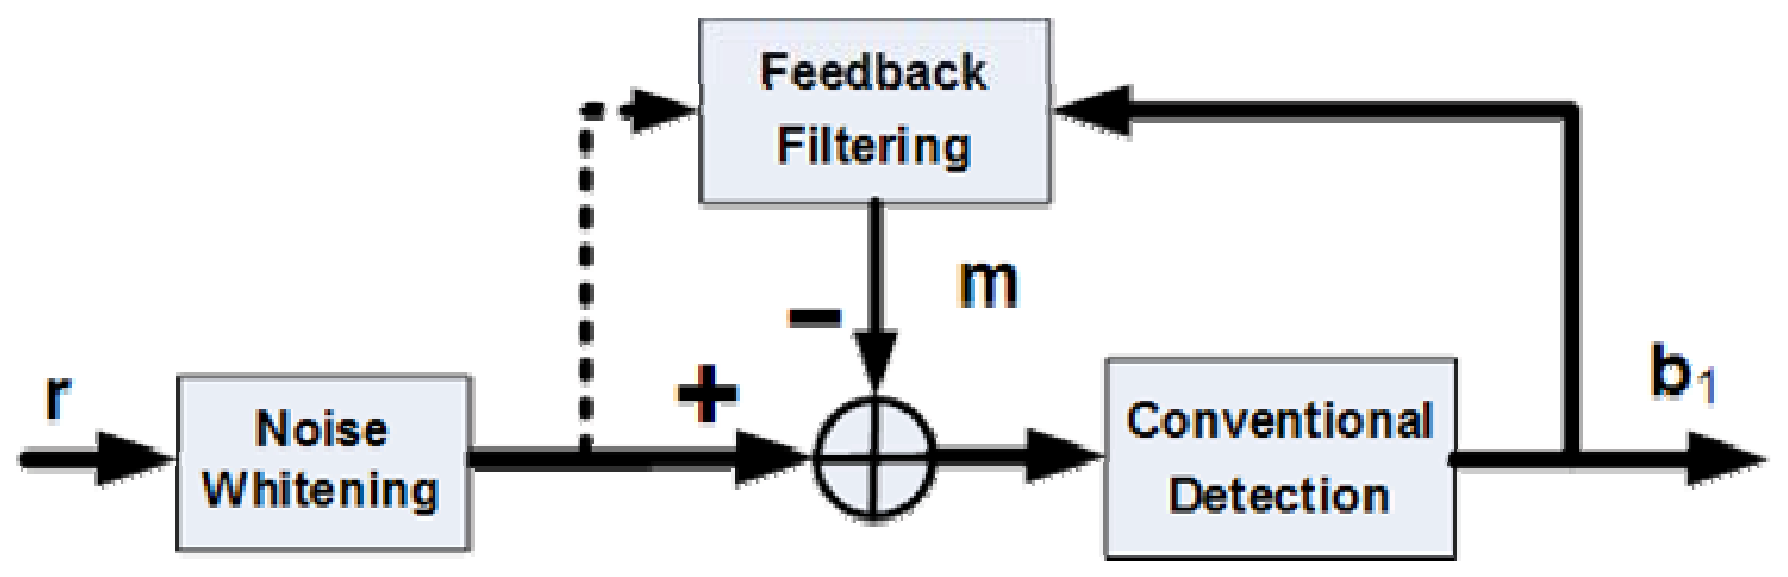
\includegraphics[width=3.2in]{BDFIC1.eps}
\caption{A group-wised decision feedback interference cancellation
block diagram} }\label{DFIC}
\end{figure}
Without loss of the generality, only the signals for the first $G$
known users are detected and their spreading signatures
$\bS_1=\left[\matrix{\bs_1&\bs_2&\ldots&\bs_G}\right]$ are known
beforehand. In order to blindly estimate MAI without knowing the
original spreading matrix $\bS$, we define a blind MAI signature
matrix
\begin{equation}
\begin{array}{rcl}
\bcS&=&\bigl[\matrix{{\br}[n-1]&{\br}[n-2]&\ldots&{\br}[n-M]}\bigr]\\
&=&\bS\bA\bB+\bN\\
&=&\bS_1\bA_1\bB_1+\bS_2\bA_2\bB_2+\bN
\end{array} \label{bcs}
\end{equation}
\noindent where $\bar\br[n-m]=\br[n-m]-\bS_1\bA_1\bb_1[n-m]$,
$m=1,\ 2,\ \ldots,\ M$ and $K\leq M+G\leq L$.
$\bB=\bigl[\bB_1^{\rm H}\ \bB_2^{\rm H}\bigr]^{\rm H}$ is the
detected data matrix for $\bcS$, $\bS_2$ is the original spreading
signature for interfering users, $\bA_1$, $\bA_2$, $\bB_1$ and
$\bB_2$ are the amplitude matrices and data matrices for desired
users and interfering users, respectively. $M=K-G$ is the minimum
number for blind interference canceller to unambiguously
distinguish different interfering signals. The relationship
between $\bcS$ and the MAI $\bm$ can be written by
\begin{equation}\hspace{-0.0in}
\begin{array}{rcl}
\bm &=&\bS_2\bA_2\bb_2\\
&=&\bigl(\bcS-\bS_1\bA_1\bB_1-\bN\bigr)\bB_2^{+}\bb_2\\
&=&\bcS\bbf-\bS_1\bD_1\bbf+\tilde{\bn}
\end{array}\label{bm}
\end{equation}
\noindent where $\bbf=\bB_2^{+}\bb_2$ denotes the projection of
$\bm$ onto the column space of $\bS_2\bA_2\bB_2$, which is similar
to $\bS_2$, $\bD_1=\bA_1\bB_1$ and
$\tilde{\bn}=-\bN\bB_2^{+}\bb_2$. With (\ref{bm}), it shows that
$\bm$ can be estimated out if $\bbf$ is known. In order to
estimate $\bbf$, we perform QR-decomposition on $\bS_1$ so that
\begin{equation}
\begin{array}{rcccl}
\bS_1&=&\bQ_1\bR_1&=&\bQ_{11}\bR_{11}
\end{array},
\end{equation}
\noindent where $\bQ_1=\left[\bQ_{11}\
\bQ_{12}\right]\in\mathbb{R}^{L\times L}$ is orthogonal and
$\bR_1=[\bR_{11}^{\rm H}\ \bzero^{\rm H}]^{\rm
H}\in\mathbb{R}^{L\times G}$, and apply $\bQ_{12}^{\rm H}$ on both
sides of (\ref{bm}). We then get
\begin{equation}
\begin{array}{rcl}
\bQ_{12}^{\rm H}\bm&=&\bQ_{12}^{\rm H}\bcS\bbf+\bQ_{12}^{\rm
H}\tilde\bn
\end{array}
\end{equation}
\noindent Since
\begin{equation}\hspace{-0.0in}
\begin{array}{rcl}
\bQ_{12}^{\rm H}\br&=&\bQ_{12}^{\rm H}\bm + \bQ_{12}^{\rm H}\bn
\end{array},
\end{equation}
\noindent $\bbf$ can be estimated from
\begin{equation}\hspace{-0.0in}
\begin{array}{rcl}
\bQ_{12}^{\rm H}\br&=&\bQ_{12}^{\rm H}\bcS\bbf+\bQ_{12}^{\rm
H}\bar\bn
\end{array},\label{f2}
\end{equation}
\noindent where $\bar\bn=\tilde\bn+\bn$.

After $\bbf$ is estimated, the MAI $\bm$ can be estimated from
(\ref{bm}) so that $\bA_1$ and $\bb_1$ can be estimated and
detected from
\begin{equation}
\begin{array}{rcl}
\br&=&\bS_1\bA_1\bb_1-\left(\bcS-\bS_1\bD_1\right)\hat{\bbf}+\bar\bn
\end{array}\label{br_bm}
\end{equation}
\noindent where $\hat{\bbf}$ is an estimate of $\bbf$. Since the
previous outputs $\bD_1$ are used for estimating interference
$\bm$ and $\bA_1$ and detecting $\bb_1$ without involving $\bS_2$,
this design framework is named blind decision-feedback
interference cancellation.

\subsection{Least Square IC}
In least square interference cancellation approaches, both the
interference $\bm$ and $\bb_1$ are estimated and detected with
least square criterion. After $\hat{\bbf}$ is known, the
interference cancellation can be done with
\begin{equation}\hspace{-0.12in}
\begin{array}{l}
\hat{\bb}_1=\mbox{arg}\min\limits_{\bx}\left\|\br-\left(\bcS_2-\bS_1\bD_1\right)\hat{\bbf}-\bS_1\hat{\bA}_1\bx\right\|_2
\end{array}.
\end{equation}
There are typically two approaches for estimating $\bbf$ with
least square criterion. One is the classic least-square approach,
which can be expressed by
\begin{equation}\hspace{-0.00in}
\begin{array}{rcl}
{\bbf}_{\rm LS}&=&\mbox{arg}\min\limits_{\bx}\left\|\bQ_{12}^{\rm
H}\br-\bQ_{12}^{\rm H}\bcS\bx\right\|_2\\
&=&\left(\bQ_{12}^{\rm H}\bcS\right)^{+}\bQ_{12}^{\rm H}\br\ .
\end{array}
\end{equation}
\noindent The LS-IC for the first $G$ users with BPSK modulation
can then be written by
\begin{equation}\hspace{-0.02in}
\begin{array}{l}
\hat{\bb}_{1\rm
LS}=\mbox{sgn}\left\{\bS_{1}^{+}\br-\bS_{1}^{+}\left(\bcS_{2}-\bS_{1}\bD_1\right)\left(\bQ_{12}^{\rm
H}\bcS\right)^{+}\bQ_{12}^{\rm H}\br\right\}
\end{array}\label{b_LS_IC}
\end{equation}
\noindent Another one is the total-least-square (TLS) approach,
which can be expressed by
\begin{equation}\hspace{-0.07in}
\begin{array}{rcl}
\left[\matrix{\hat{\bY}\cr{\bbf}_{\rm
TLS}}\right]&=&\mbox{arg}\min\limits_{\bY\
\bx}\left\|\left[\matrix{\bQ_{12}^{\rm H}\bcS\cr\bQ_{12}^{\rm
H}\br}\right]-\left[\matrix{\bY\cr\bY\bx}\right]\right\|_2
\end{array}.
\end{equation}
\noindent If $\sigma_{K-G}'>\sigma_{K-G+1}$, the TLS estimation of
$\bbf$ is~\cite{Huff91}
\begin{equation}\hspace{-0.070in}
\begin{array}{l}
{\bbf_{\rm TLS}}=\left(\bcS^{\rm H}\bQ_{12}\bQ_{12}^{\rm
H}\bcS-\sigma_{K-G+1}^{2}\bI\right)^{-1}\bcS^{\rm
H}\bQ_{12}\bQ_{12}^{\rm H}\br
\end{array}
\end{equation}
\noindent where $\sigma_{K-G}'$ and $\sigma_{K-G+1}$ are the
$(K-G)$th and $(K-G+1)$th largest singular value of $\bQ_{12}^{\rm
H}\bcS$ and $\bQ_{12}^{\rm H}\left[\matrix{\br&\bcS}\right]$. And
the TLS-IC for BPSK modulation can be expressed by
\begin{equation}\hspace{0.0in}
\begin{array}{l}
\hat{\bb}_{1\rm
TLS}=\mbox{sgn}\left\{\bS_{1}^{+}\br-\bS_{1}^{+}\left({\bcS}_{2}-{\bS}_{1}{\bD_1}\right){\bbf_{\rm
TLS}}\right\}
\end{array}\label{b_TLS_IC}
\end{equation}

\subsection{Minimum Mean-Square Error IC}
In MMSE-based approach,the interference cancellation is done with
solving
\begin{equation}\hspace{-0.15in}
\begin{array}{l}
\hat{\bb}_1=\mbox{arg}\min\limits_{\bx}\mbox{E}\left\|\br-\left(\bcS_2-\bS_1\bD_1\right)\hat{\bbf}-\bS_1\hat{\bA}_1\bx\right\|_2
\end{array}
\end{equation}
\noindent providing $\hat{\bbf}$ is known. On the other hand,
$\bbf$ is estimated with minimizing MSE
\begin{equation}\hspace{-0.08in}
\begin{array}{rcl}
{\bbf}_{\rm
MMSE}&=&\mbox{arg}\min\limits_{\bx}\mbox{E}\left\|\bQ_{12}^{\rm
H}\br-\bQ_{12}^{\rm H}\bcS\bx\right\|_2^2\\
&=&\left(\bcS^{\rm H}\bQ_{12}\bQ_{12}^{\rm
H}\bcS-\sigma^{2}\bI\right)^{-1}\bcS^{\rm H}\bQ_{12}\bQ_{12}^{\rm
H}\br
\end{array}
\end{equation}
\noindent so that the MMSE-IC for BPSK modulation can be written
by
\begin{equation}\hspace{-0.10in}
\begin{array}{l}
\hat{\bb}_1=\\
\mbox{sgn}\left\{\left(\bS_1\hat{\bA}_1^2\bS_1^{\rm
H}-\sigma^2\bI\right)^{+}\bS_1^{\rm
H}\left[\br-\left(\bcS_2-\bS_1\bD_1\right){\bbf}_{\rm
MMSE}\right]\right\}.
\end{array}
\end{equation}


\section{Performance Analysis}

\subsection{Relationship with Blind MUD}

It can be proven that the LS-IC in (\ref{b_LS_IC}) actually is
equal to the blind LS decorrelating detector
\begin{equation}
\begin{array}{rcl}
\hat{\bb}_{1}&=&\mbox{sgn}\left\{\left[\matrix{\bI&\bB_1}\right]\bA\bbf_{\rm
LS}\right\}
\end{array}
\end{equation}
\noindent with respect to
\begin{equation}
\begin{array}{rcl}
{\bbf}_{\rm
LS}&=&\matrix{\mbox{arg}\min\limits_{\bx}\left\|\br-\left[\matrix{\bS_1&\bcS}\right]\bx\right\|_2^2}
\end{array}
\label{LSProb}
\end{equation}
\noindent and MMSE-IC is equal to the blind MMSE detector
\begin{equation}\hspace{0.0in}
\begin{array}{rcl}
\hat{\bb}_1&=&\mbox{sgn}\left\{\left[\matrix{\bI&\bB_1}\right]\bA\bbf_{\rm
MMSE}\right\}
\end{array}
\end{equation}
\noindent with respect to
\begin{equation}
\begin{array}{rcl}
{\bbf}_{\rm
MMSE}&=&\mbox{arg}\min\limits_{\bx}\mbox{E}\left\|\br-\left[\matrix{\bS_1&\bcS}\right]\bx\right\|_2^2
\end{array}.
\end{equation}

\subsection{AME and Near-Far Resistance}
A commonly used performance measure for a multiuser detector is
asymptotic multiuser efficiency (AME) and near-far
resistance~\cite{Verd98}. Since the proposed algorithms converges
to the conventional decorrelating detector as $\sigma^2\rightarrow
0$, their AME and near-far resistance are identical to the
decorrelating detector:
\begin{equation}
\begin{array}{rcl}
\bar{\eta}_k&=&\frac{1}{\left[\bR^{+}\right]_{kk}}
\end{array}.
\end{equation}
\subsection{CRLB for $\bbf$ Estimation}
The Cram\'{e}r-Rao Lower Bound (CRLB) is given by the inverse of
the Fisher information matrix (FIM). Providing the blind spreading
matrix $\bcS$ is known beforehand, we first define the parameter
vector $\mathbf{\phi} = \left[\bar{\sigma}^{2}\ \bbf^{\rm
H}\right]^{\rm H}$, where $\bar{\sigma}^{2}
=(1+\frac{M-G}{M-K})\sigma^{2}$, for computing the FIM
\begin{equation}
\begin{array}{rcl}
{\bI(\mathbf{\phi})} &=& {\rm E} \left\{ \left( \frac{\partial
\ln{\cal L}}{\partial \mathbf{\phi}} \right) \left( \frac{\partial
\ln{\cal L}}{\partial \mathbf{\phi}} \right)^{\rm H} \right\}
\label{fim}
\end{array}
\end{equation}
\noindent where $\ln{\cal L}$ is the log-likelihood function given
by
\begin{equation}
\begin{array}{rcl}
\ln{\cal
L}&=&C-L\ln\bar{\sigma}^2-\frac{1}{2\bar{\sigma}^2}\parallel\mathbf{e}\parallel_2^2
\end{array},\label{logl}
\end{equation}
\noindent $C$ is a constant and
$\mathbf{e}=\bT\bQ_1\br-\bcR_{22}\bbf$. Providing $\bcS$ is known,
the closed-form CRLB expression of $\bbf$ is then given by
\begin{equation}
\begin{array}{rcl}
{\rm CRLB}(\bbf\ |\ \bcS) &
=&(1+\frac{M-G}{M-K})\sigma^{2}(\bcR_{22}^{\rm H}\bcR_{22})^{\rm
+}
\end{array}.\label{CRLB_f}
\end{equation}
\noindent It shows that the accuracy of estimating $\bbf$ may
increase with increasing $M$.
\subsection{Bit-Error Rate}

\section{Computer Simulations}
There are $K=10$ users with the group size $G=3$ and the spreading
sequences used in simulations are $64$-chip ($L=64$) random
sequences. In the computer simulations, the previous amplitude
estimation from (\ref{A_estimation}) is directly use for the next
detection without any amplitude filtering. From Subplot (a) in
Fig. 3, it is interesting to see that the performance of the
simplest LS detector has the best performance. From Subplot (b),
it is very impressive to find that the performance of blind LS
detector is very close to the conventional decorrelating detector
whatever how strong the MAI is in our simulations when $M$ is
large enough. We then check the performance of the proposed LS
blind detector against the amplitude estimation errors. From Fig.
4, we can see that the BER of the LS detector basically is
unchanged against amplitude estimation error when SNR is large
enough. From Fig. 5, we can see that the performance of the LS
detector can be better providing $M$ is larger enough. This
confirms (\ref{noise_var_new}), which shows that the variance of
$\bar{\bn}$ decrease with increasing $M$.
\begin{figure} \center{
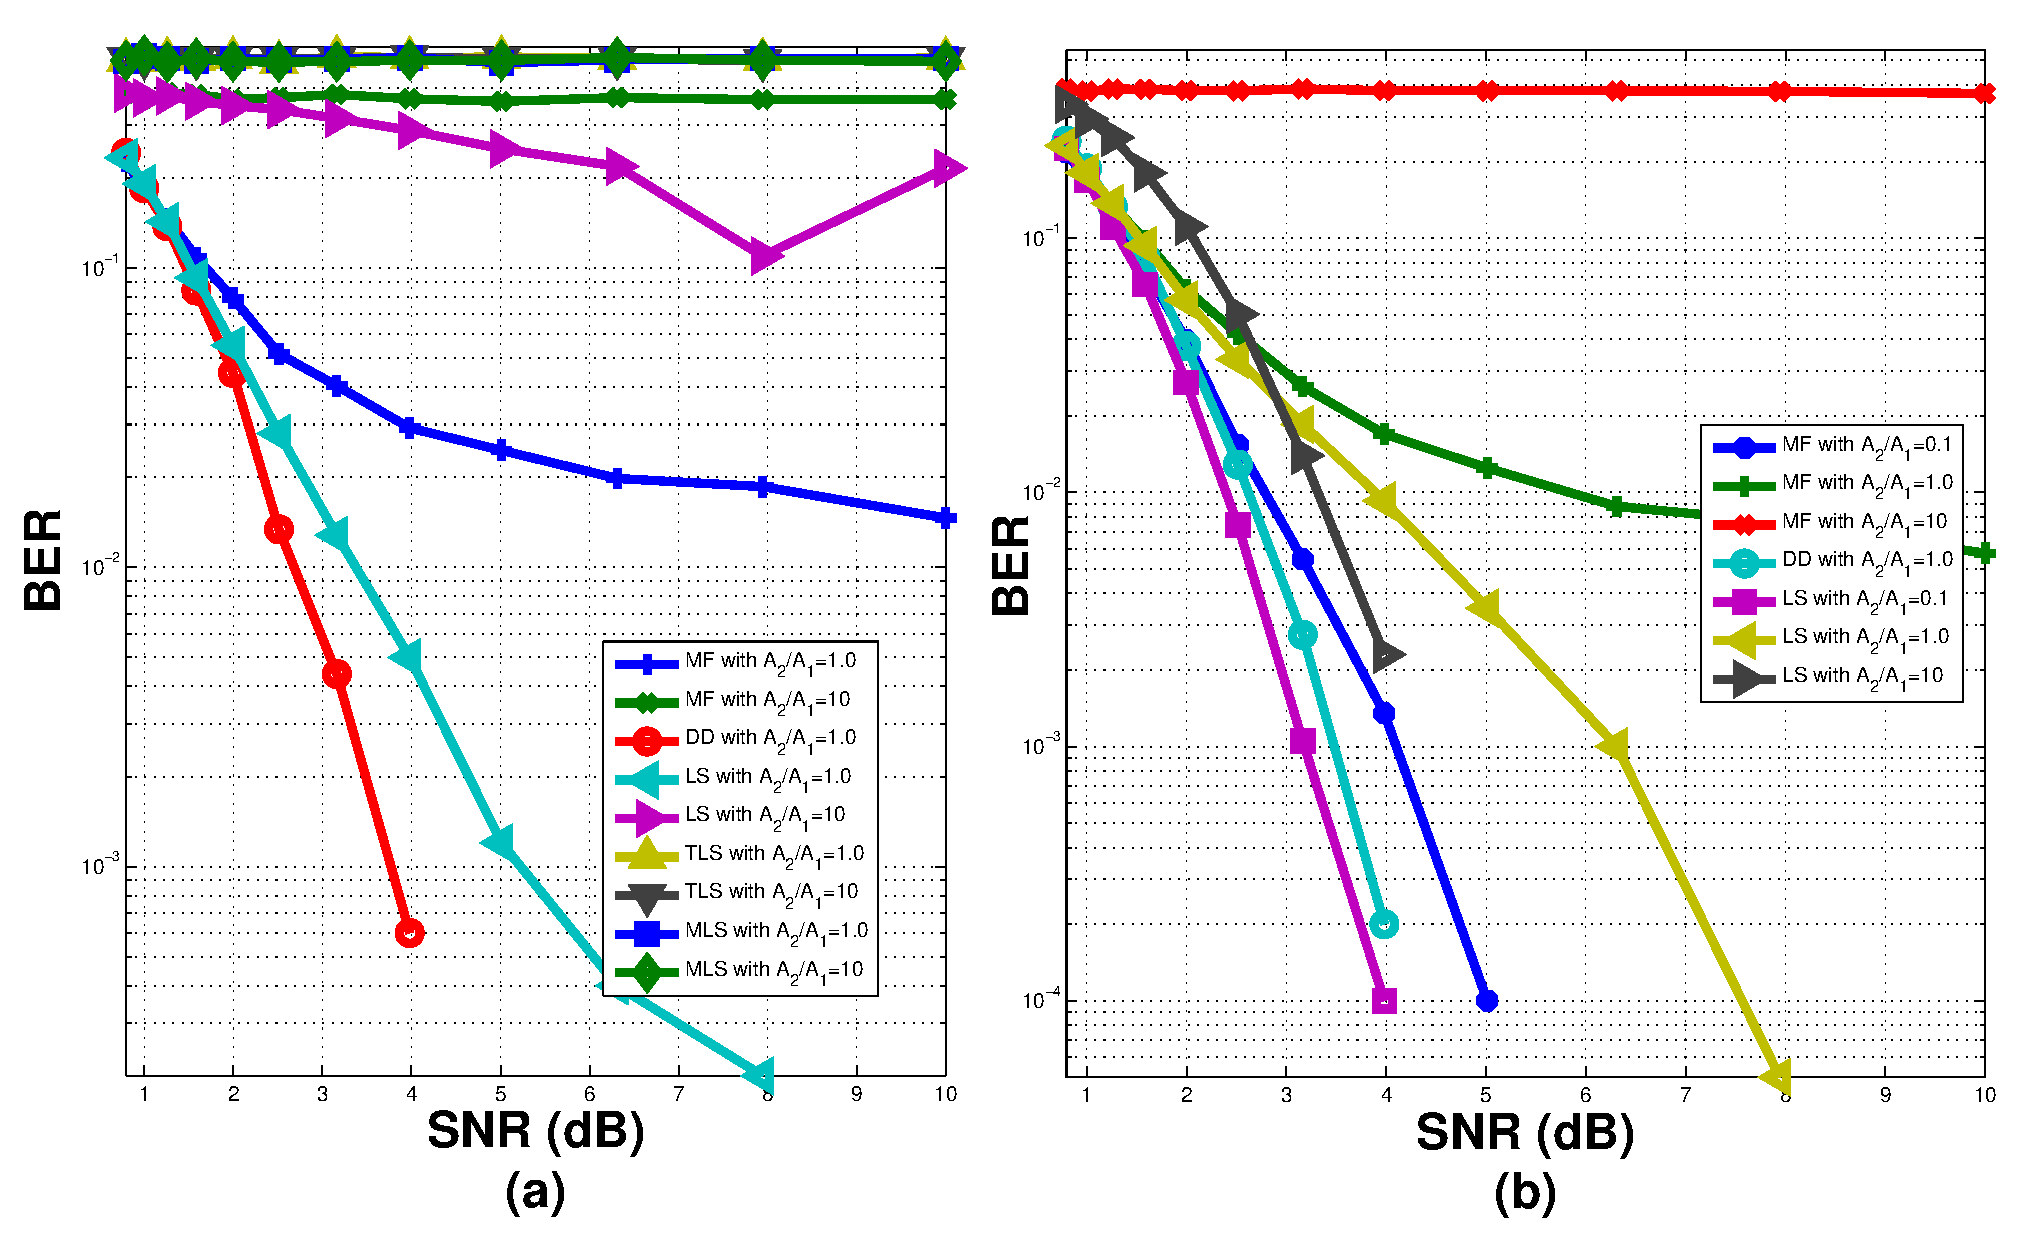
\includegraphics[width=3in]{BER_SNR_10_64.eps}
\caption{ (a) The performance of the proposed blind MUDs against
SNR, $M=12$. (b) The performance of the proposed blind LS
detector, $M=63$. } }\label{BER_SNR}
\end{figure}
\begin{figure} \center{
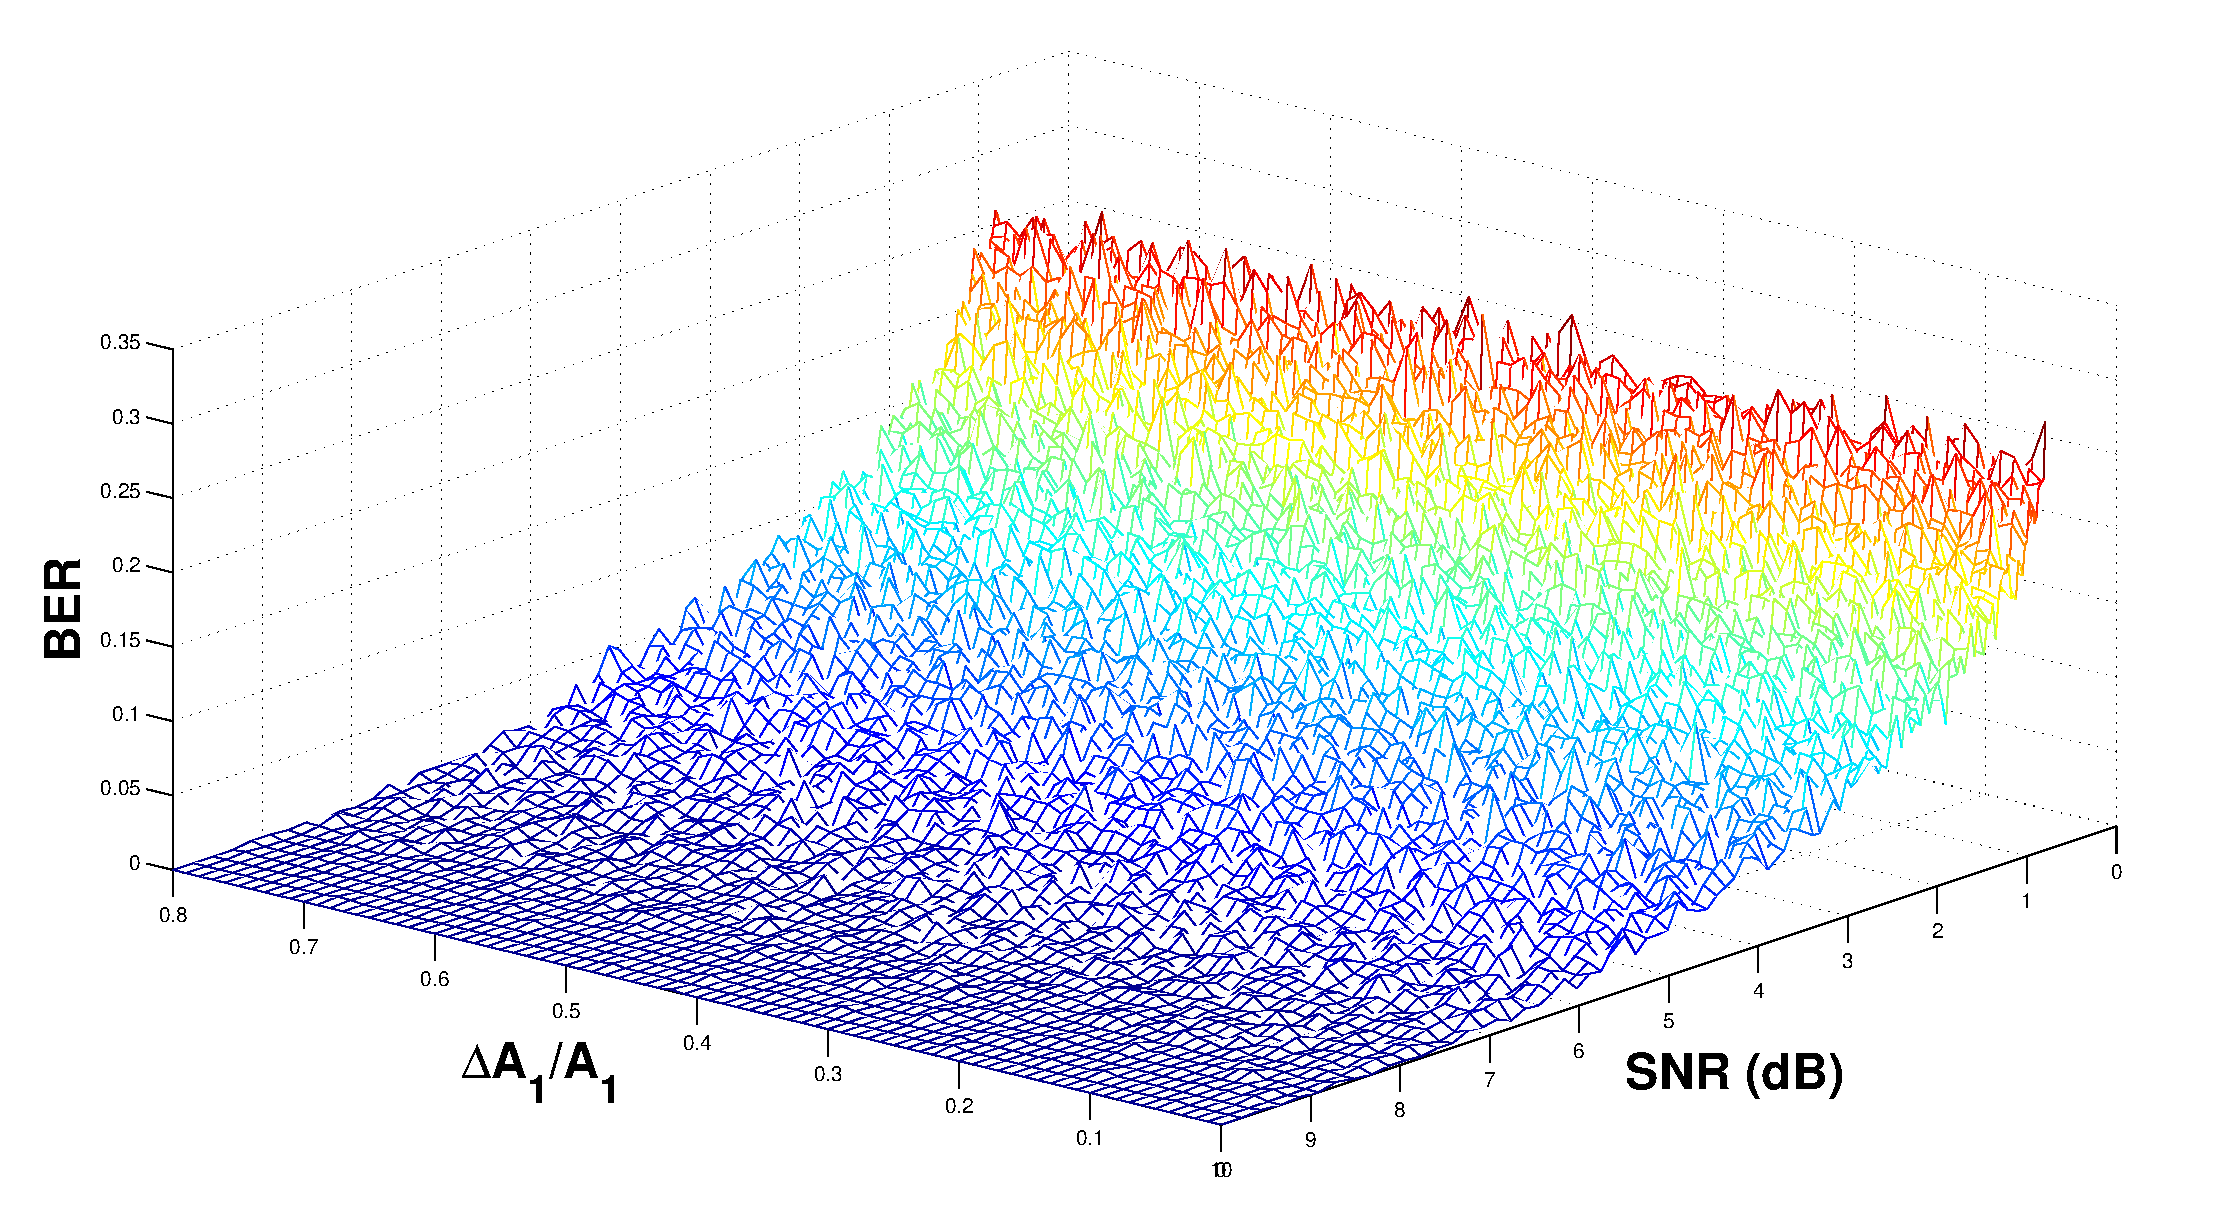
\includegraphics[width=2.5in]{BER_A_SNR_10_64_LSs.eps}
\caption{ The performance of the LS detector against amplitude
estimation error ${\Delta}{A_1}/A_1$ and SNR, $M=63$.}
}\label{BER_A_SNR}
\end{figure}
\begin{figure}
\center{
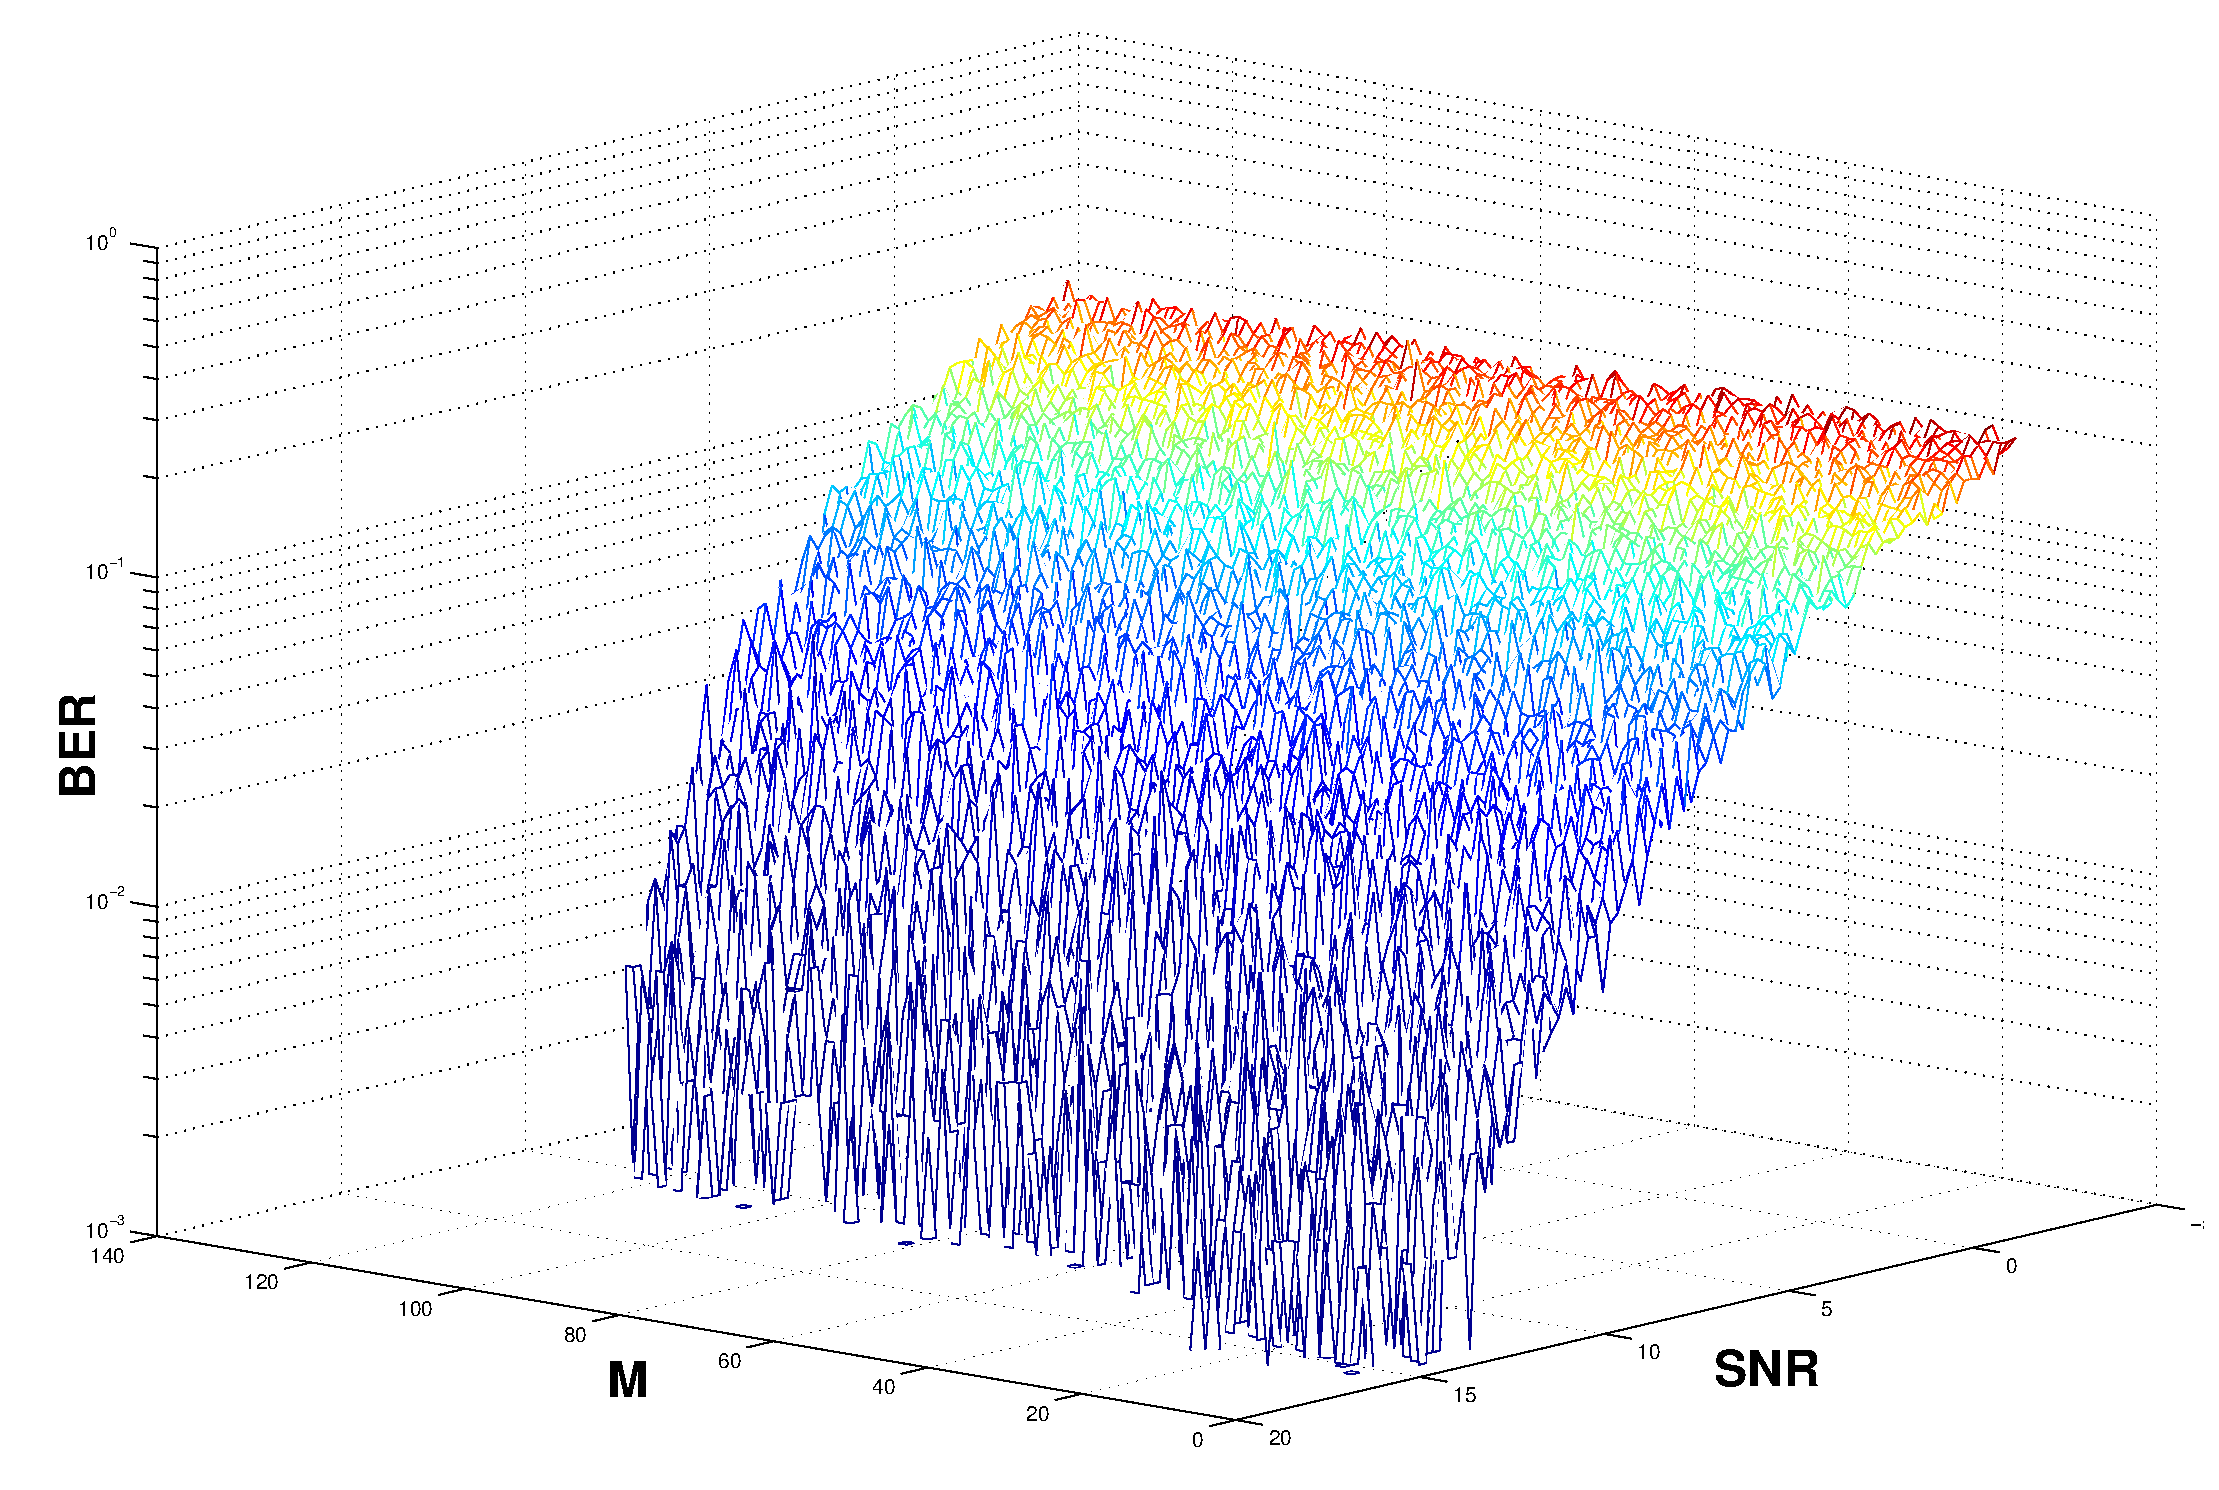
\includegraphics[width=2.5in]{BER_M_SNR_10_64_LSs.eps}
\caption{ The performance of the LS blind MUD against $M$ and
SNR.} }\label{BER_M_SNR}
\end{figure}
\section{Conclusions}
In this paper, we proposed a blind multiuser detection framework
as well as several blind detectors. The proposed blind detectors
are direct and simple without any channel or spreading sequence
estimation or subspace separation operation. \small
\bibliographystyle{unsrt}
\bibliography{FastBDD,InterferenceCancellation}
\end{document}
